Chapter~\ref{chap:crosssubject} establishes that on unseen participants the learned
fusion heads lose to parameter-free softmax averaging, and that the loss is
concentrated in the vision modality. This chapter asks whether that failure is a
property of the fusion operator or of the representation it receives. The answer is
the principal new contribution of this thesis: a label-free, per-participant
normalisation of the fusion input, computed from a short unlabelled calibration
recording, lifts every learned fusion head from below naive late fusion to 11--14
percentage points above it, and the effect holds with as few as twenty calibration
clips. Section~\ref{sec:cal_mechanism} shows that what the normalisation removes is
linearly decodable participant identity.

\section{Hypothesis}
\label{sec:cal_hypothesis}

A learned fusion head is fitted to features from the training participants. If
those features encode each participant as a distinct offset in feature space---a
characteristic mean and spread per dimension---then two things follow. First, the
head can partly solve its training task by exploiting that offset, as the
within-subject encoders were shown to do in Chapter~\ref{chap:crosssubject}. Second,
a held-out participant arrives at an offset the head has never seen, so its inputs
lie off the training distribution in a direction that carries no emotional
information. Naive late fusion is immune to the second effect, because it combines
class probabilities rather than features and contains no fitted quantity that the
offset can mislead.

If this account is right, removing each participant's own offset---without using any
labels---should restore the learned heads' advantage. If instead the learned heads
fail because single-token attention and MLP fusion cannot extract more than averaging
does from these encoders, normalisation should make little difference.

\section{Method: Per-Participant Feature Standardisation}
\label{sec:cal_method}

Let $x^{(m)}_{s,t} \in \mathbb{R}^{d_m}$ be the pre-classifier feature of modality
$m \in \{a, v, e\}$ for trial $t$ of participant $s$, produced by the fold's encoder.
The default protocol of Chapter~\ref{chap:crosssubject} standardises every
participant with one mean and variance estimated on the training participants. The
calibrated protocol instead standardises each participant with their own statistics:
\begin{equation}
  \tilde{x}^{(m)}_{s,t} = \frac{x^{(m)}_{s,t} - \mu^{(m)}_{s}}{\sigma^{(m)}_{s} + \epsilon},
  \qquad
  \mu^{(m)}_{s} = \frac{1}{|C_s|}\sum_{t \in C_s} x^{(m)}_{s,t},
  \label{eq:subjnorm}
\end{equation}
where $\sigma^{(m)}_{s}$ is the per-dimension standard deviation over the same set,
$\epsilon = 10^{-6}$, and $C_s$ is the participant's \emph{calibration set}. The
statistics use features only; no emotion label enters Equation~\ref{eq:subjnorm}.

Training participants are normalised with $C_s$ equal to all of their trials. The
fusion heads---cross-attention, concat-MLP and softhard modality dropout---are then
retrained on the normalised features with exactly the Stage~C recipe of
Chapter~\ref{chap:crosssubject}: the same folds, the same encoders and cached
features, the same inner-validation participants for epoch selection, and the same
hyperparameters. Only the normalisation changes.

For held-out participants, two settings are evaluated:
\begin{itemize}
  \item \textbf{Transductive.} $C_s$ is all 400 of the participant's trials,
  including the trials that are then scored. This is the simplest form of the method
  and is reported first, but it uses the scored trials' features to compute the
  statistics.
  \item \textbf{Disjoint calibration.} $C_s$ is a set of $n$ trials drawn from the
  participant, and accuracy is measured only on the remaining $400 - n$ trials. This
  models the deployable version: a new user records a short unlabelled session, and
  every later prediction is normalised with statistics from that session.
\end{itemize}

Naive late fusion and the unimodal classifiers operate on encoder logits rather than
on the fusion features, so the normalisation does not change them; they appear with
the same values as in Chapter~\ref{chap:crosssubject}. Section~\ref{sec:cal_fairness}
discusses what this means for the comparison.

\section{Results: Transductive Calibration}
\label{sec:cal_transductive}

Table~\ref{tab:cal_main} reports the 42-participant results. Confidence intervals are
10{,}000-sample bootstrap intervals over participants \cite{Efron1993Bootstrap}; tests
are paired Wilcoxon signed-rank \cite{Wilcoxon1945} with Holm correction
\cite{Holm1979} over the eight comparisons of the family.

\begin{table}[htbp]
\centering
\small
\caption{Cross-subject accuracy with per-participant calibration (transductive), 42
participants. $\Delta$ is the mean paired difference from naive late fusion;
``better'' counts participants for whom the head beats naive late fusion. Holm
correction over the 8 tests of Table~\ref{tab:cal_ranking} and this table.}
\label{tab:cal_main}
\begin{tabular}{lccccc}
\hline
\textbf{Method} & \textbf{Mean} & \textbf{95\% CI} & \textbf{$\Delta$ vs naive} & \textbf{Better} & \textbf{$p_{\mathrm{Holm}}$} \\
\hline
Concat-MLP              & 75.93\% & [73.5, 78.2] & $+13.78$ pp & 41/42 & $1.3\times10^{-7}$ \\
Modality dropout (full) & 75.02\% & [72.6, 77.3] & $+12.86$ pp & 42/42 & $1.3\times10^{-7}$ \\
Cross-attention         & 73.87\% & [71.4, 76.3] & $+11.71$ pp & 40/42 & $1.8\times10^{-7}$ \\
Modality dropout (AV)   & 73.57\% & [71.2, 75.9] & $+11.42$ pp & 40/42 & $1.4\times10^{-7}$ \\
Naive late fusion       & 62.15\% & [59.4, 64.9] & ---          & ---   & --- \\
\hline
\end{tabular}
\end{table}

Every learned head now exceeds naive late fusion, by 11.4 to 13.8 percentage points,
on at least 40 of the 42 participants. The same heads scored 57.6--58.8\% under the
default normalisation (Table~\ref{tab:cs_main}); calibration therefore moves each of
them by 15.7 to 17.1 points, from 3--4.5 points \emph{below} naive late fusion to
11--14 points above it. Table~\ref{tab:cal_effect} gives the per-head change.

\begin{table}[htbp]
\centering
\small
\caption{Effect of calibration on each learned head (same encoders, same folds, same
training recipe; only the normalisation differs). Every one of the 42 participants
improves under every head; Holm correction over the four tests.}
\label{tab:cal_effect}
\begin{tabular}{lcccc}
\hline
\textbf{Head} & \textbf{Default} & \textbf{Calibrated} & \textbf{Change} & \textbf{$p_{\mathrm{Holm}}$} \\
\hline
Concat-MLP              & 58.80\% & 75.93\% & $+17.13$ pp & $6.6\times10^{-8}$ \\
Modality dropout (full) & 58.77\% & 75.02\% & $+16.24$ pp & $6.6\times10^{-8}$ \\
Cross-attention         & 57.61\% & 73.87\% & $+16.26$ pp & $6.6\times10^{-8}$ \\
Modality dropout (AV)   & 57.89\% & 73.57\% & $+15.68$ pp & $6.6\times10^{-8}$ \\
\hline
\end{tabular}
\end{table}

\subsection{Fold Consistency}

Table~\ref{tab:cal_perfold} reports the pooled accuracy of each fold. The gain is
present in every fold: the smallest margin of any head over naive late fusion in any
fold is 5.1 points (modality dropout evaluated without EEG, fold 2), and the largest is 19.9 points
(concat-MLP, fold 1).

\begin{table}[htbp]
\centering
\small
\caption{Per-fold accuracy under transductive calibration. Every held-out
participant contributes 400 trials, so pooled accuracy equals the participant mean.}
\label{tab:cal_perfold}
\begin{tabular}{lccccc}
\hline
\textbf{Method} & \textbf{Fold 0} & \textbf{Fold 1} & \textbf{Fold 2} & \textbf{Fold 3} & \textbf{Fold 4} \\
\hline
Concat-MLP              & 0.738 & 0.815 & 0.720 & 0.753 & 0.767 \\
Modality dropout (full) & 0.736 & 0.806 & 0.719 & 0.735 & 0.751 \\
Cross-attention         & 0.720 & 0.784 & 0.710 & 0.733 & 0.743 \\
Modality dropout (AV)   & 0.724 & 0.792 & 0.706 & 0.721 & 0.730 \\
Naive late fusion       & 0.629 & 0.616 & 0.655 & 0.586 & 0.621 \\
\hline
\end{tabular}
\end{table}

\subsection{Ranking of the Fusion Heads}
\label{sec:cal_ranking}

Under the default normalisation the three learned heads were statistically
indistinguishable (Table~\ref{tab:cs_wilcoxon}). Under calibration they separate
(Table~\ref{tab:cal_ranking}).

\begin{table}[htbp]
\centering
\small
\caption{Pairwise comparisons of the calibrated heads (paired Wilcoxon, Holm over
the same 8-test family as Table~\ref{tab:cal_main}).}
\label{tab:cal_ranking}
\begin{tabular}{llccc}
\hline
\textbf{Head A} & \textbf{Head B} & \textbf{$\Delta$} & \textbf{A better} & \textbf{$p_{\mathrm{Holm}}$} \\
\hline
Concat-MLP              & Modality dropout (full) & $+0.92$ pp & 27/42 & $0.031$ \\
Concat-MLP              & Cross-attention         & $+2.07$ pp & 36/42 & $1.1\times10^{-5}$ \\
Modality dropout (full) & Cross-attention         & $+1.15$ pp & 27/42 & $0.0058$ \\
Modality dropout (full) & Modality dropout (AV)   & $+1.45$ pp & 34/42 & $7.0\times10^{-5}$ \\
\hline
\end{tabular}
\end{table}

The ordering is concat-MLP $>$ modality dropout $>$ cross-attention, and each step is
significant. Two readings matter for the thesis title. First, attention-based fusion
is not the strongest operator on this representation: a two-layer MLP over the
concatenated features beats it by 2.1 points. Second, softhard modality dropout
recovers more than half of that gap for the same attention architecture (1.15 of the
2.07 points), leaving the attention model 0.92 points behind concat-MLP. This matches
the within-subject leak-free result of Chapter~\ref{chap:within}, where dropout and
concat-MLP were tied and both beat plain cross-attention: under both protocols,
training discipline matters more than the choice of fusion operator.

The last row bears on robustness. Under calibration, zeroing EEG at inference costs
the dropout model 1.45 points, a significant loss; under the default normalisation
the same comparison cost 0.89 points and was not significant
(Section~\ref{sec:cs_discussion}). Calibration therefore makes EEG's contribution to
the fused prediction measurable on unseen participants, although it remains the
smallest of the three.

\subsection{Per-Class Effect}
\label{sec:cal_perclass}

Table~\ref{tab:cal_perclass} reports per-class recall pooled over all 16{,}800
held-out trials, together with macro-averaged $F_1$.

\begin{table}[htbp]
\centering
\small
\caption{Per-class recall and macro-$F_1$ on all held-out trials, default versus
calibrated normalisation. Naive late fusion is unaffected by calibration.}
\label{tab:cal_perclass}
\begin{tabular}{llcccccc}
\hline
\textbf{Protocol} & \textbf{Method} & \textbf{Neu.} & \textbf{Sad.} & \textbf{Ang.} & \textbf{Hap.} & \textbf{Calm.} & \textbf{Macro-$F_1$} \\
\hline
Either     & Naive late fusion & 0.689 & 0.620 & 0.765 & 0.650 & 0.384 & 0.615 \\
\hline
Default    & Concat-MLP        & 0.656 & 0.536 & 0.687 & 0.696 & 0.365 & 0.582 \\
           & Modality dropout  & 0.639 & 0.562 & 0.724 & 0.660 & 0.354 & 0.581 \\
           & Cross-attention   & 0.652 & 0.557 & 0.706 & 0.605 & 0.361 & 0.571 \\
\hline
Calibrated & Concat-MLP        & 0.776 & 0.721 & 0.847 & 0.835 & 0.618 & 0.758 \\
           & Modality dropout  & 0.782 & 0.732 & 0.823 & 0.834 & 0.580 & 0.748 \\
           & Cross-attention   & 0.763 & 0.712 & 0.818 & 0.822 & 0.578 & 0.737 \\
\hline
\end{tabular}
\end{table}

Calibration raises recall on every class for every head. The largest change is on
Calmness, the hardest class under every protocol: concat-MLP moves from 0.365 to
0.618, and all three heads gain more than 21 points on it. Calmness is the
lowest-arousal state in the EAV schema and the one most easily confused with Neutral
(Section~\ref{sec:per_class_results}); a participant-specific resting offset is
exactly the kind of nuisance that would blur a low-arousal distinction, and removing
it helps that class most. Macro-$F_1$ rises from 0.571--0.582 to 0.737--0.758, so the
accuracy gain is not bought by favouring the majority classes.

\section{Results: Disjoint Calibration}
\label{sec:cal_disjoint}

The transductive result has two properties a sceptical reader will object to. It
computes each held-out participant's statistics from the very trials it then scores,
and it relies on a hidden prior: every EAV participant contributes exactly 80 trials
per class, so their mean is a perfectly class-balanced average. A real calibration
session need not be balanced. The disjoint study addresses both
(\texttt{calibration\_study.py}).

\textbf{Protocol.} The heads trained in Section~\ref{sec:cal_transductive} are used
unchanged. For each held-out participant, $n \in \{5, 10, 20, 50, 100, 200\}$
calibration trials are drawn, the statistics of Equation~\ref{eq:subjnorm} are
computed from them alone, and accuracy is measured on the remaining $400-n$ trials.
Naive late fusion is scored on exactly the same evaluation trials, so every
comparison is paired. Each cell is repeated with five random seeds and averaged per
participant before testing. Calibration trials are drawn three ways:
\begin{itemize}
  \item \textbf{Random:} uniformly at random. This uses no labels at all.
  \item \textbf{Neutral-only:} Neutral-cued trials only, modelling an instructed
  ``sit neutrally for a minute'' session. At most 80 such trials exist, so $n \le 50$.
  \item \textbf{Skewed:} class proportions drawn from a Dirichlet(0.3) distribution,
  producing strongly unbalanced sessions. This is a stress test of the class-balance
  prior.
\end{itemize}
Each EAV trial is a five-second segment, so $n$ trials correspond to $5n$ seconds of
recording: 20 trials are 100 seconds. Holm correction is applied over all 68
head-versus-naive tests of the study.

\begin{table}[htbp]
\centering
\small
\caption{Disjoint random calibration: accuracy on the $400-n$ trials not used for
calibration, mean over 42 participants (each averaged over 5 seeds). The
transductive row ($n = 400$) is Table~\ref{tab:cal_main}.}
\label{tab:cal_random}
\begin{tabular}{rcccccc}
\hline
\textbf{$n$} & \textbf{Seconds} & \textbf{Naive} & \textbf{Concat-MLP} & \textbf{Dropout} & \textbf{Cross-attn} & \textbf{Dropout (AV)} \\
\hline
5   & 25    & 62.15\% & 67.11\% & 66.95\% & 66.22\% & 65.73\% \\
10  & 50    & 62.13\% & 71.86\% & 71.08\% & 70.55\% & 69.91\% \\
20  & 100   & 62.14\% & 73.84\% & 73.04\% & 72.48\% & 71.84\% \\
50  & 250   & 62.17\% & 75.08\% & 74.25\% & 73.42\% & 72.85\% \\
100 & 500   & 62.03\% & 75.66\% & 74.72\% & 73.96\% & 73.45\% \\
200 & 1000  & 62.44\% & 75.81\% & 75.09\% & 74.02\% & 73.59\% \\
\hline
400 & (all) & 62.15\% & 75.93\% & 75.02\% & 73.87\% & 73.57\% \\
\hline
\end{tabular}
\end{table}

\begin{figure}[htbp]
\centering
\IfFileExists{images/fig_cal_curve.png}{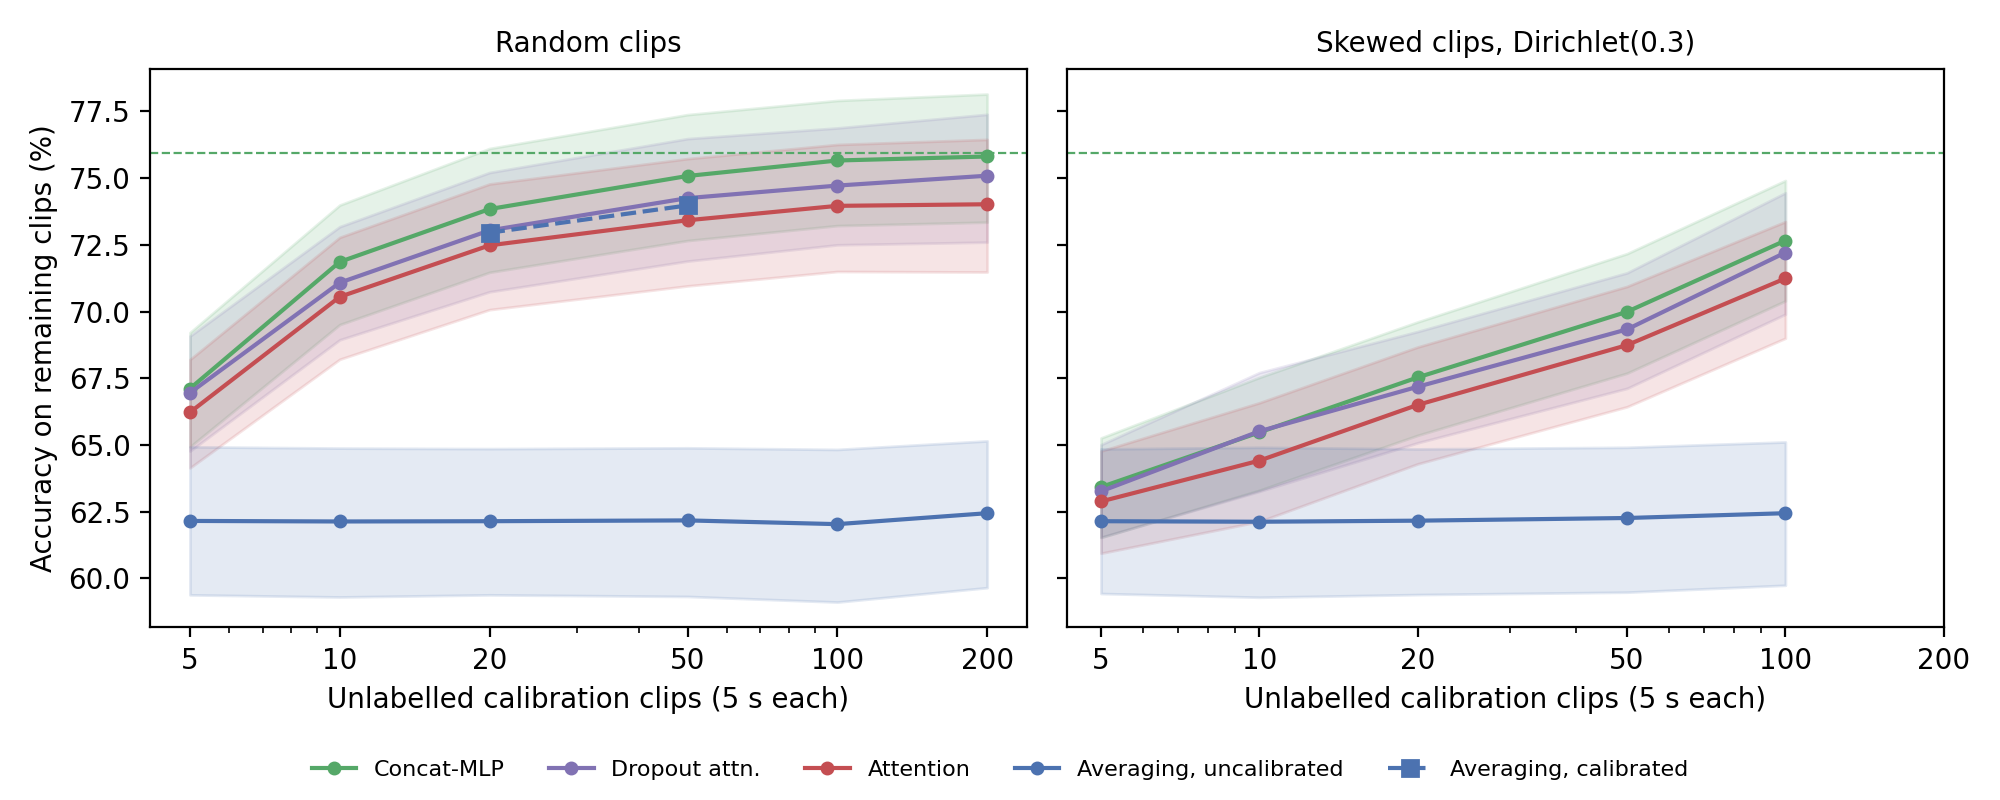
\includegraphics[width=0.85\textwidth]{images/fig_cal_curve.png}}{\fbox{\parbox{0.8\textwidth}{\centering Missing image placeholder: \texttt{images/fig\_cal\_curve.png} (accuracy versus $n$ calibration trials, random and skewed conditions, with bootstrap CIs, from \texttt{p3\_stats/calibration\_curve.csv}).}}}
\caption{Accuracy on non-calibration trials as a function of the number of unlabelled
calibration trials. Naive late fusion is flat because it does not use the
calibration statistics.}
\label{fig:cal_curve}
\end{figure}

Three results follow from Table~\ref{tab:cal_random} and Table~\ref{tab:cal_delta}.

\textbf{The gain survives disjoint calibration.} With 20 random trials---100 seconds
of unlabelled recording---every head beats naive late fusion by 9.7 to 11.7 points,
all significant after correction. Transductive calibration is therefore not the
source of the effect; it is simply the $n = 400$ end of the curve.

\textbf{The curve saturates by about 50 trials.} At $n = 50$ concat-MLP reaches
75.08\%, within 0.9 points of the transductive 75.93\%, and further calibration adds
little. At $n = 10$ all four heads are already significantly above naive late fusion.
At $n = 5$ only concat-MLP and the dropout model are; five trials give too noisy an
estimate of a 768- or 960-dimensional mean and variance for the attention heads.

\textbf{The ranking of the heads is preserved at every $n$}: concat-MLP $>$ dropout
$>$ cross-attention $>$ dropout (AV).

\begin{table}[htbp]
\centering
\small
\caption{Gain over naive late fusion (percentage points) for each calibration
condition and size. $^{*}$: significant after Holm correction over all 68 tests.
$^{\dagger}$: fewer than 42 participants contributed valid draws; not interpretable
(see text).}
\label{tab:cal_delta}
\begin{tabular}{lrcccc}
\hline
\textbf{Condition} & \textbf{$n$} & \textbf{Concat-MLP} & \textbf{Dropout} & \textbf{Cross-attn} & \textbf{Dropout (AV)} \\
\hline
Random  & 5   & $+4.96^{*}$  & $+4.80^{*}$  & $+4.07$      & $+3.58$ \\
        & 10  & $+9.73^{*}$  & $+8.94^{*}$  & $+8.42^{*}$  & $+7.77^{*}$ \\
        & 20  & $+11.69^{*}$ & $+10.89^{*}$ & $+10.34^{*}$ & $+9.69^{*}$ \\
        & 50  & $+12.91^{*}$ & $+12.08^{*}$ & $+11.25^{*}$ & $+10.68^{*}$ \\
        & 100 & $+13.63^{*}$ & $+12.70^{*}$ & $+11.93^{*}$ & $+11.42^{*}$ \\
        & 200 & $+13.38^{*}$ & $+12.65^{*}$ & $+11.58^{*}$ & $+11.15^{*}$ \\
\hline
Neutral & 5   & $-3.52$ & $-3.67$ & $-3.55$ & $-3.45$ \\
        & 10  & $-1.82$ & $-2.14$ & $-2.33$ & $-1.82$ \\
        & 20  & $+0.08$ & $-0.24$ & $-0.18$ & $-0.12$ \\
        & 50  & $+4.09$ & $+4.04$ & $+3.99$ & $+4.03$ \\
\hline
Skewed  & 5   & $+1.28$      & $+1.13$      & $+0.75$      & $-0.09$ \\
        & 10  & $+3.34$      & $+3.38$      & $+2.29$      & $+2.20$ \\
        & 20  & $+5.37^{*}$  & $+5.03$      & $+4.34$      & $+3.83$ \\
        & 50  & $+7.73^{*}$  & $+7.07^{*}$  & $+6.48^{*}$  & $+6.08^{*}$ \\
        & 100 & $+10.22^{*}$ & $+9.77^{*}$  & $+8.80^{*}$  & $+8.76^{*}$ \\
        & 200$^{\dagger}$ & $+15.04$ & $+12.75$ & $+12.42$ & $+10.33$ \\
\hline
\end{tabular}
\end{table}

\subsection{Robustness to the Composition of the Calibration Session}
\label{sec:cal_robustness}

\textbf{Neutral-only calibration fails.} Calibrating on Neutral trials alone never
produces a significant gain. At $n = 5$ and $n = 10$ every head falls below naive late
fusion, at $n = 20$ they are tied, and at $n = 50$ the $+4$-point gain is not
significant. The mechanism is visible in Equation~\ref{eq:subjnorm}: the statistics
are meant to estimate the participant's overall feature mean, but a Neutral-only
session estimates the Neutral class mean instead. Subtracting it shifts every
emotional trial by that trial's class's difference from Neutral, which is emotional
signal, not identity. The practical consequence is concrete: an instructed ``relax
and look at the camera'' enrolment session is the wrong design for this method.

\textbf{Unbalanced sessions need more data.} Under Dirichlet(0.3) sessions, which are
frequently dominated by one or two classes, the gain is significant for every head
only from $n = 50$ (250 seconds), and reaches 8.8--10.2 points at $n = 100$. A
skewed session biases the mean in the same way as a Neutral-only one but less
severely, and averaging over more trials dilutes the bias.

\textbf{The skewed $n = 200$ cell is excluded.} A draw is rejected when the sampled
proportions require more than the 80 trials available in some class. At $n = 200$ many
draws are rejected, the surviving draws are biased toward balanced compositions, and
fewer than 42 participants contribute; the cell is flagged in
\texttt{calibration\_curve.csv} and is not interpreted.

Taken together, the robustness conditions turn the method into a specification: the
calibration session should contain roughly 50 unlabelled clips, about four minutes,
of \emph{varied} emotional content---for example, an unscripted conversation---rather
than an instructed neutral baseline.

\section{Mechanism: What Calibration Removes}
\label{sec:cal_mechanism}

The hypothesis of Section~\ref{sec:cal_hypothesis} makes a testable prediction: the
fusion features should encode participant identity under the default normalisation,
and that identity should disappear under calibration. Two linear probes test this
directly (\texttt{identity\_probe.py}). Linear probes are deliberate: they measure
what is linearly available in a representation, not what a flexible model could
extract. Each is trained for a fixed number of full-batch steps with no epoch
selection.

\textbf{Probe A---identity.} A 42-way linear classifier predicts \emph{which
participant} a trial came from, trained on a random half of every participant's
trials and scored on the other half (chance $1/42 = 2.4\%$). Under calibration the
normalisation statistics are computed from the probe's training half only; computing
them from all trials would make the two halves' means mirror each other and push the
probe below chance, overstating the removal (Section~\ref{sec:p3_challenges}).

\textbf{Probe B---emotion, cross-subject.} A five-way linear classifier trained on
each fold's training participants and scored on its held-out participants, one
accuracy per participant.

\begin{table}[htbp]
\centering
\small
\caption{Linear probes on the fold encoders' features, mean over the five folds.
Probe A: 42-way participant identity (chance 2.4\%). Probe B: 5-way emotion on
held-out participants (chance 20\%), with the number of participants improved and a
paired Wilcoxon test.}
\label{tab:identity_probe}
\begin{tabular}{lcccccc}
\hline
& \multicolumn{2}{c}{\textbf{Probe A: identity}} & \multicolumn{4}{c}{\textbf{Probe B: emotion (cross-subject)}} \\
\textbf{Modality} & \textbf{Default} & \textbf{Calibrated} & \textbf{Default} & \textbf{Calibrated} & \textbf{Gain} & \textbf{Improved} \\
\hline
Audio  & 97.0\%  & 2.5\% & 58.6\% & 67.8\% & $+9.2$ pp  & 41/42 \\
Vision & 100.0\% & 2.5\% & 38.9\% & 52.5\% & $+13.6$ pp & 41/42 \\
EEG    & 81.6\%  & 2.4\% & 35.4\% & 45.5\% & $+10.1$ pp & 40/42 \\
\hline
\end{tabular}
\end{table}

\begin{figure}[htbp]
\centering
\IfFileExists{images/fig_identity_probe.png}{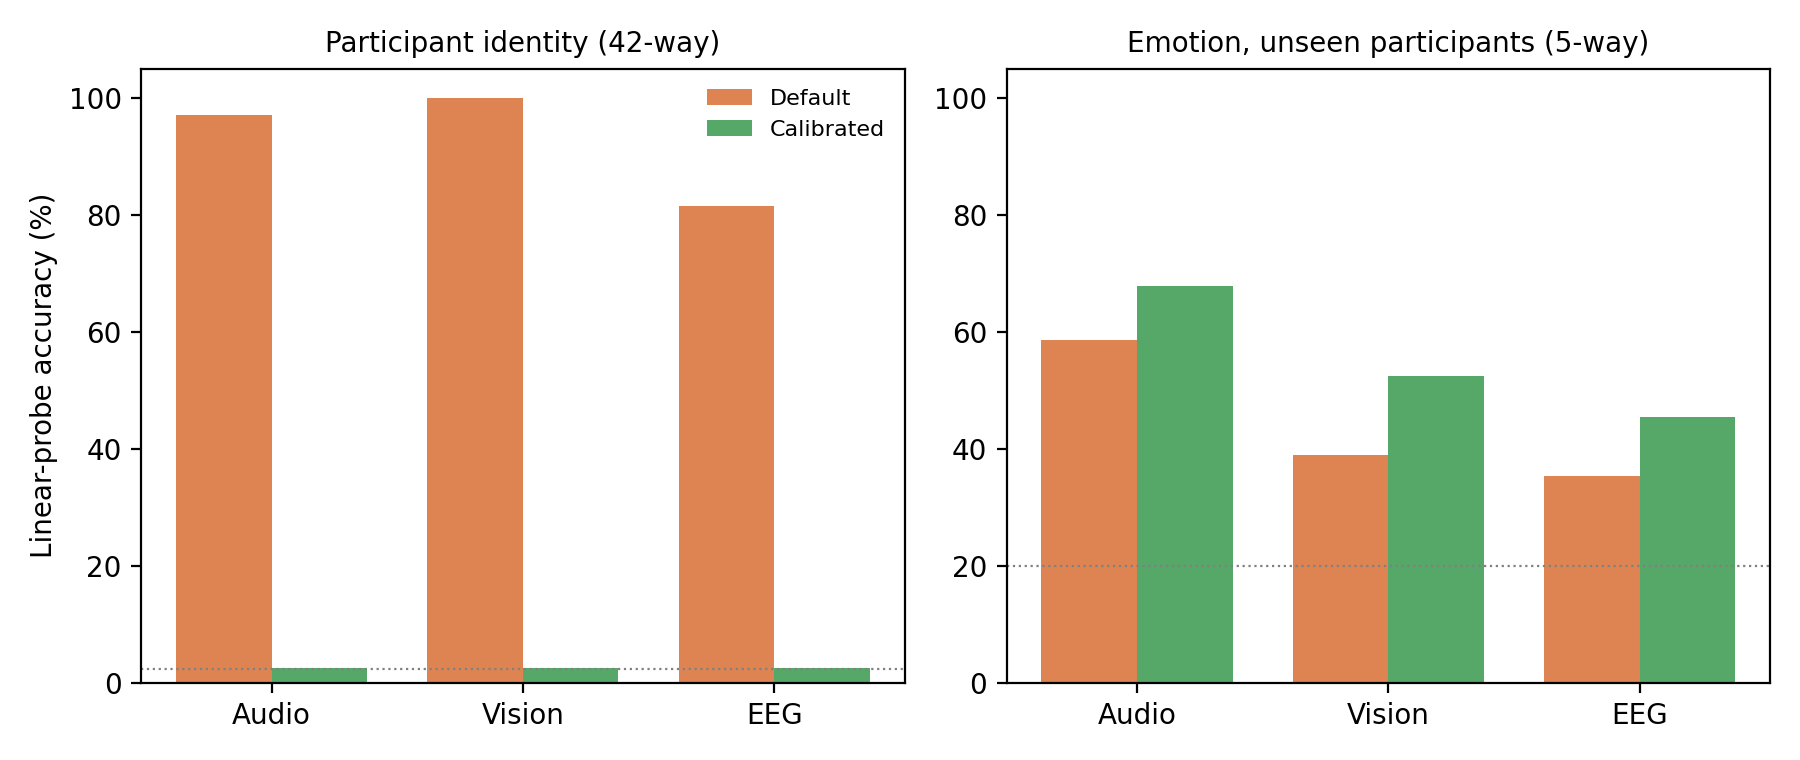
\includegraphics[width=0.95\textwidth]{images/fig_identity_probe.png}}{\fbox{\parbox{0.9\textwidth}{\centering Missing image placeholder: \texttt{images/fig\_identity\_probe.png} (run \texttt{make\_p3\_figures.py}).}}}
\caption{Linear probes before and after per-participant calibration. Left: participant identity (chance 2.4\%, dotted). Right: emotion on unseen participants (chance 20\%).}
\label{fig:identity_probe}
\end{figure}

Table~\ref{tab:identity_probe} and Figure~\ref{fig:identity_probe} support the hypothesis on both counts. Under the
default normalisation, participant identity is linearly decodable from every
modality: essentially perfectly from vision (100.0\%), almost perfectly from audio
(97.0\%), and at 81.6\% from EEG, against a chance rate of 2.4\%. After calibration
all three fall to chance. At the same time, cross-subject emotion decoding improves
for every modality, on 40 or more of the 42 participants in each case (paired Wilcoxon, all
$p < 10^{-4}$ uncorrected and below $10^{-3}$ after Holm correction over the three
tests). Vision, the modality
that collapsed in Chapter~\ref{chap:crosssubject}, gains most ($+13.6$ points).

Two qualifications keep this reading honest.

First, the removal of identity is partly true by construction. Equation~\ref{eq:subjnorm}
removes each participant's per-dimension mean and variance, which are exactly the
cues a linear identity classifier would use. Identity carried in higher-order
structure---for example, in the covariance between dimensions---could survive, and a
non-linear probe might still recover it. The supported claim is therefore that
calibration removes the \emph{linearly available, first- and second-moment} identity
signal, and that this is sufficient to produce the gains above; it is not that the
features become identity-free.

Second, identity being present does not by itself predict transfer failure. Audio
features are 97\% identity-decodable, yet audio transferred at parity in
Chapter~\ref{chap:crosssubject}. What distinguishes vision is not \emph{whether}
identity is present but how entangled it is with the emotion decision: the vision
encoder's emotion boundary is drawn partly along identity directions, so a new face
lands on the wrong side of it. Probe B is consistent with this: vision gains the most
from removing identity because its emotion signal depended on identity the most.

\section{Alternatives That Do Not Work}
\label{sec:cal_negative}

Before calibration was tested, a more direct reading of the thesis title was
evaluated: if learned heads fail because their modality weighting is fitted to the
training participants, perhaps a \emph{dynamic} weighting computed per trial from
each modality's own confidence would transfer better, since it contains no fitted
parameters (\texttt{dynamic\_late\_fusion.py}). All variants were scored on the
default-normalisation cross-subject logits.

\textbf{Confidence is informative.} Splitting each modality's held-out predictions
into confidence quintiles, accuracy in the most confident fifth exceeds the least
confident fifth by 46 points for audio, 31 for vision and 29 for EEG. Confidence is
therefore a usable signal.

\textbf{Confidence weighting does not help.} Weighting each modality's softmax by
its maximum probability, negative entropy or top-two margin, raised to the powers 1,
2 or 4, or selecting the single most confident modality, lowers accuracy in every
case, by 1.05 to 3.77 points relative to naive late fusion (Table~\ref{tab:dynamic}).
The reason is that mean-softmax averaging is \emph{already} confidence-weighted: a
confident modality contributes a peaked distribution that dominates the average.
Explicit reweighting counts confidence twice and hands more control to over-confident
modalities.

\textbf{Temperature scaling does not help either.} Fitting one temperature per
modality on the inner-validation participants \cite{Guo2017Calibration} gives mean
temperatures of 2.00 (audio), 1.49 (vision) and 1.72 (EEG)---every encoder is
over-confident on unseen participants---but temperature-scaled late fusion scores
62.46\%, $+0.30$ points over naive late fusion and not significant ($p = 0.16$, 23 of
42 participants improved).

\begin{table}[htbp]
\centering
\small
\caption{Dynamic (per-trial, confidence-weighted) late fusion on default-normalised
cross-subject logits, paired against naive late fusion ($n = 42$). $p$-values are
uncorrected; this was an exploratory family and no variant improves on the baseline.}
\label{tab:dynamic}
\begin{tabular}{lccc}
\hline
\textbf{Scheme} & \textbf{Mean} & \textbf{$\Delta$ vs naive} & \textbf{$p$} \\
\hline
Temperature-scaled late fusion           & 62.46\% & $+0.30$ pp & 0.16 \\
Naive late fusion                        & 62.15\% & ---        & --- \\
Max-probability weighting                & 61.11\% & $-1.05$ pp & 0.010 \\
Negative-entropy weighting               & 60.99\% & $-1.16$ pp & 0.027 \\
Max-probability weighting, power 4       & 59.68\% & $-2.48$ pp & 0.0007 \\
Margin weighting                         & 59.59\% & $-2.57$ pp & 0.0001 \\
Most-confident modality only             & 58.54\% & $-3.62$ pp & $<10^{-4}$ \\
Margin weighting, power 4                & 58.38\% & $-3.77$ pp & $<10^{-4}$ \\
\hline
\end{tabular}
\end{table}

The contrast with Section~\ref{sec:cal_transductive} is the point. Adapting the
\emph{decision} per trial does nothing; adapting the \emph{input space} per participant
recovers 15.7--17.1 points. The useful form of dynamic fusion on unseen participants is
not reweighting modalities by confidence but giving a learned fusion operator---of
which attention is one---inputs from which the participant has been removed.

\section{Fairness of the Comparison and Limitations}
\label{sec:cal_fairness}

\textbf{The baseline was not calibrated.} Naive late fusion combines encoder logits,
which Equation~\ref{eq:subjnorm} does not touch, so the 11--14-point margin is the
margin of calibrated learned fusion over \emph{uncalibrated} averaging. An analogous
per-participant correction of the encoder logits was not evaluated, and it is the most
direct open question this chapter leaves. The calibrated linear probes of
Table~\ref{tab:identity_probe} give a partial reference point: the best calibrated
single-modality probe (audio, 67.8\%) is 8.1 points below the calibrated concat-MLP
head (75.9\%). That gap is between means from different model classes and was not
tested as a paired comparison, but it indicates that calibrated fusion is doing more
than calibrating its best input.

\textbf{Enrolment is required.} The method needs a short unlabelled recording from
each new user before it can normalise their predictions. This is weaker than one-shot
inference on a single clip, and the assumption must be stated with any deployment
claim. It is, however, label-free, and the recording can be the first few minutes of
use.

\textbf{Same-session calibration.} Calibration and evaluation trials come from the same
EAV recording session. Whether statistics from one session transfer to another day,
with different electrode placement, lighting or microphone position, is untested.

\textbf{Training-side normalisation is transductive.} Training participants are
normalised with all of their trials. Only the held-out side was varied in the
disjoint study.

\section{Answer to RQ8}
\label{sec:cal_rq}

\textbf{RQ8---Subject calibration:} Yes. A label-free, per-participant standardisation
of the fusion features lifts every learned fusion head from 57.6--58.8\% to
73.6--75.9\% on unseen participants, 11.4--13.8 points above naive late fusion
($p_{\mathrm{Holm}} < 2\times10^{-7}$, at least 40 of 42 participants improved). The
effect needs about 20 unlabelled calibration clips (100 seconds) to be significant for
every head and saturates at about 50; the session must contain varied emotional
content, since Neutral-only calibration fails and strongly unbalanced sessions need
50--100 clips. The mechanism is the removal of linearly decodable participant
identity, which falls from 82--100\% to chance. Under calibration the learned heads
separate significantly---concat-MLP $>$ modality dropout $>$ cross-attention---so
attention-based fusion beats averaging decisively once identity is removed, but it is
not the strongest operator, and modality-dropout training is what makes it
competitive.
